\documentclass{article}
\usepackage{graphicx}
\usepackage[left=1in,right=1in]{geometry}

\title{Comment Mutations}
\author{Lorenzo Rosset}
\date{\today}

\begin{document}

\maketitle

\section{Azoarcus}
\begin{figure}[h]
    \centering
    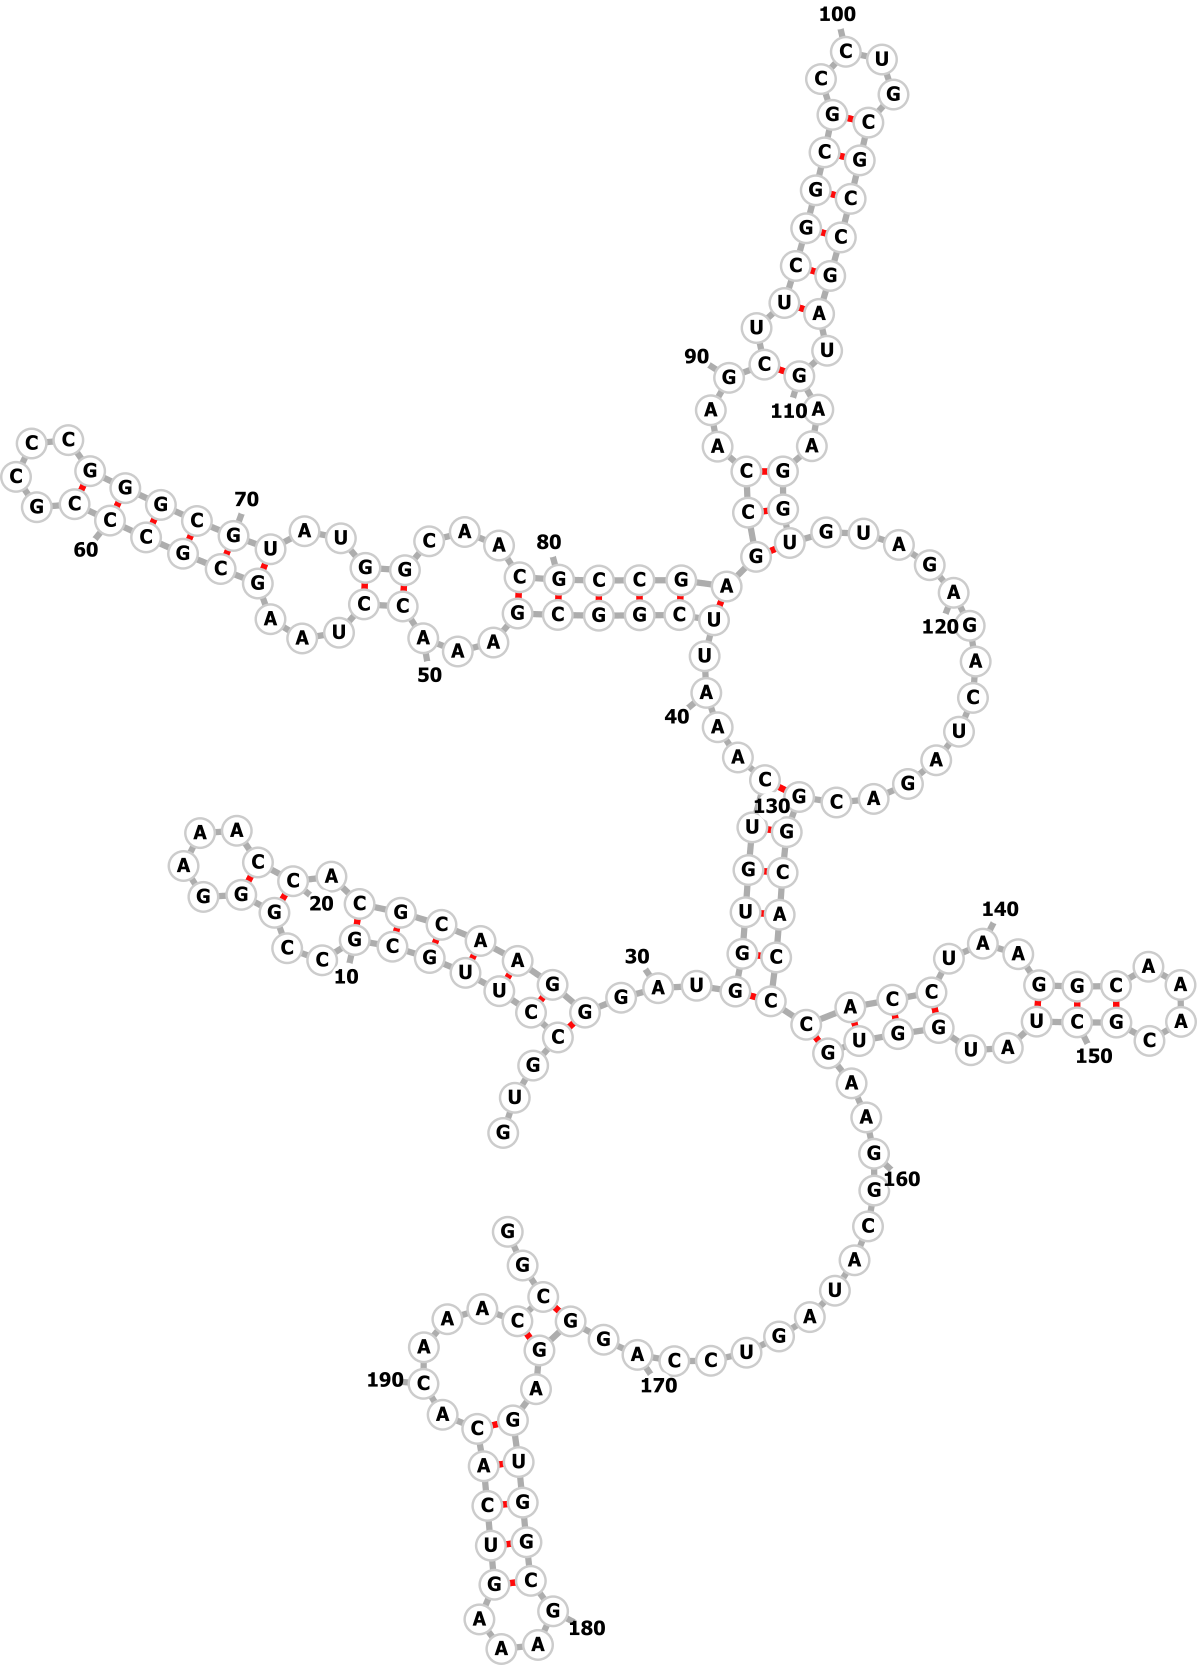
\includegraphics[width=0.5\textwidth]{figures/forna_azoarcus.png}
    \caption{Azoarcus visualized using the consensus secondary structure.}
    \label{fig:structure azoarcus}
\end{figure}

\section{Wild-type 5}
\begin{figure}[h]
    \centering
    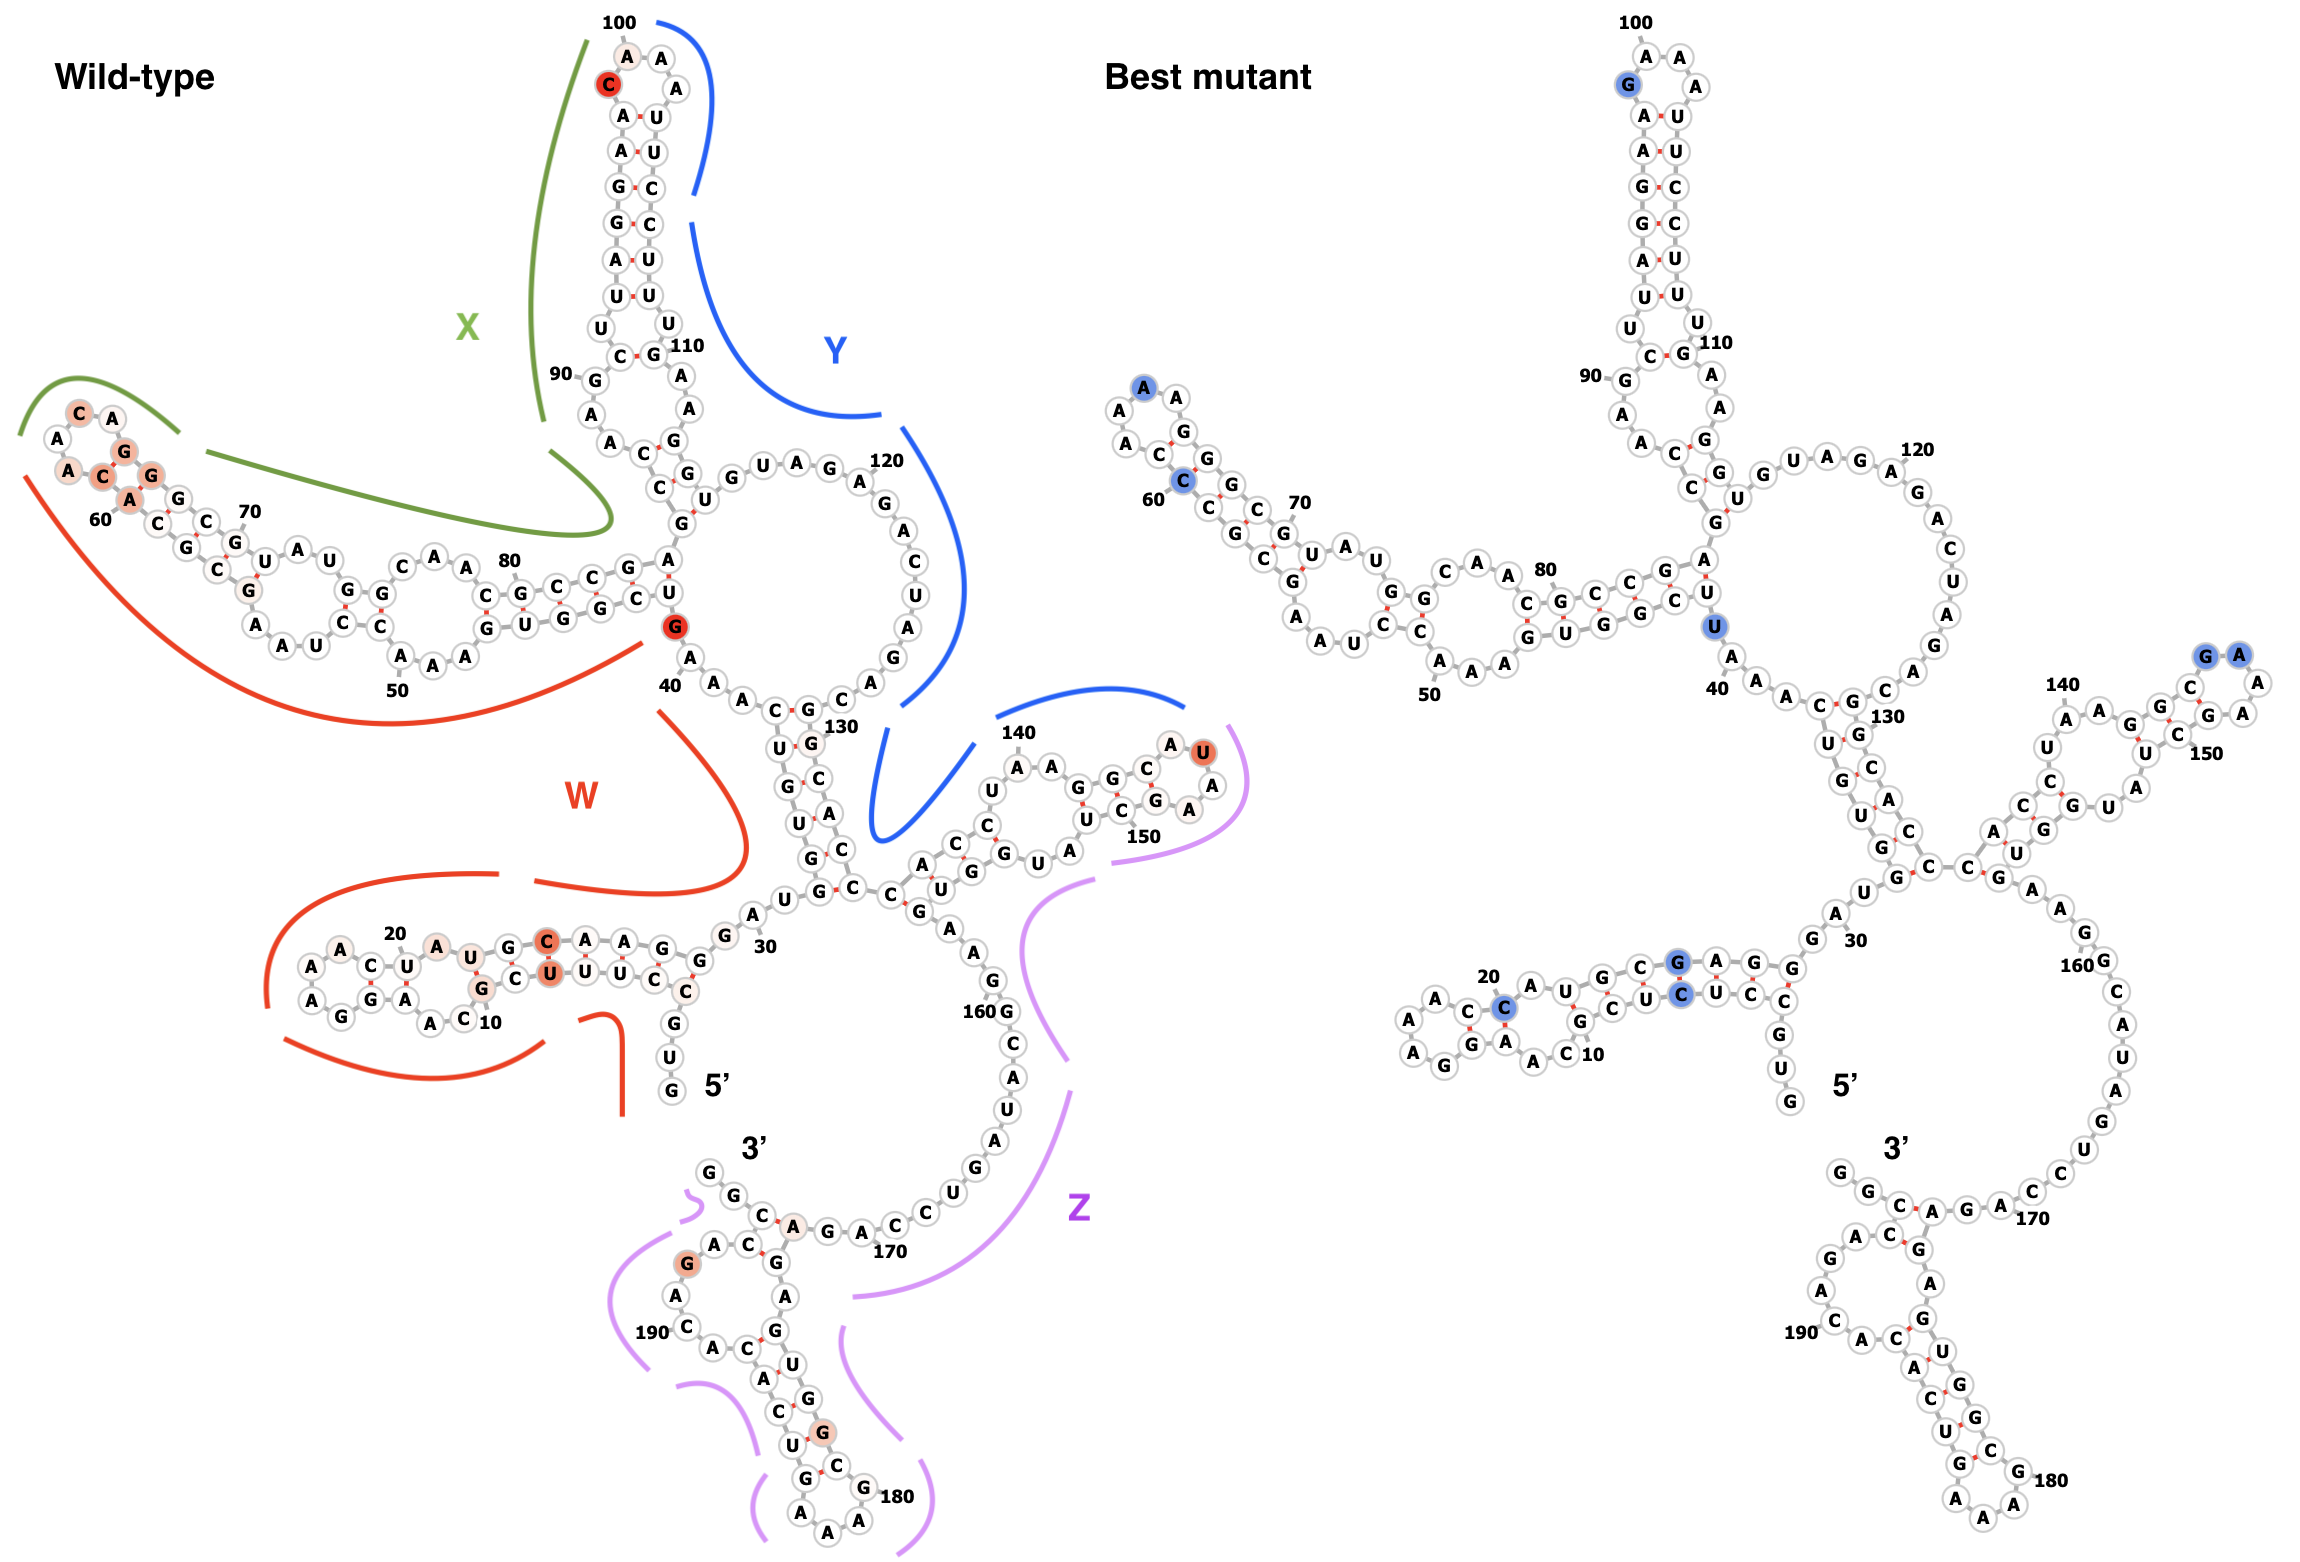
\includegraphics[width=\textwidth]{figures/forna_wt_5.png}
    \caption{Wild-type 5 (left) and the best mutant (right) visualized using the consensus secondary structure.}
    \label{fig:structure wt_5}
\end{figure}

\begin{figure}[h]
    \centering
    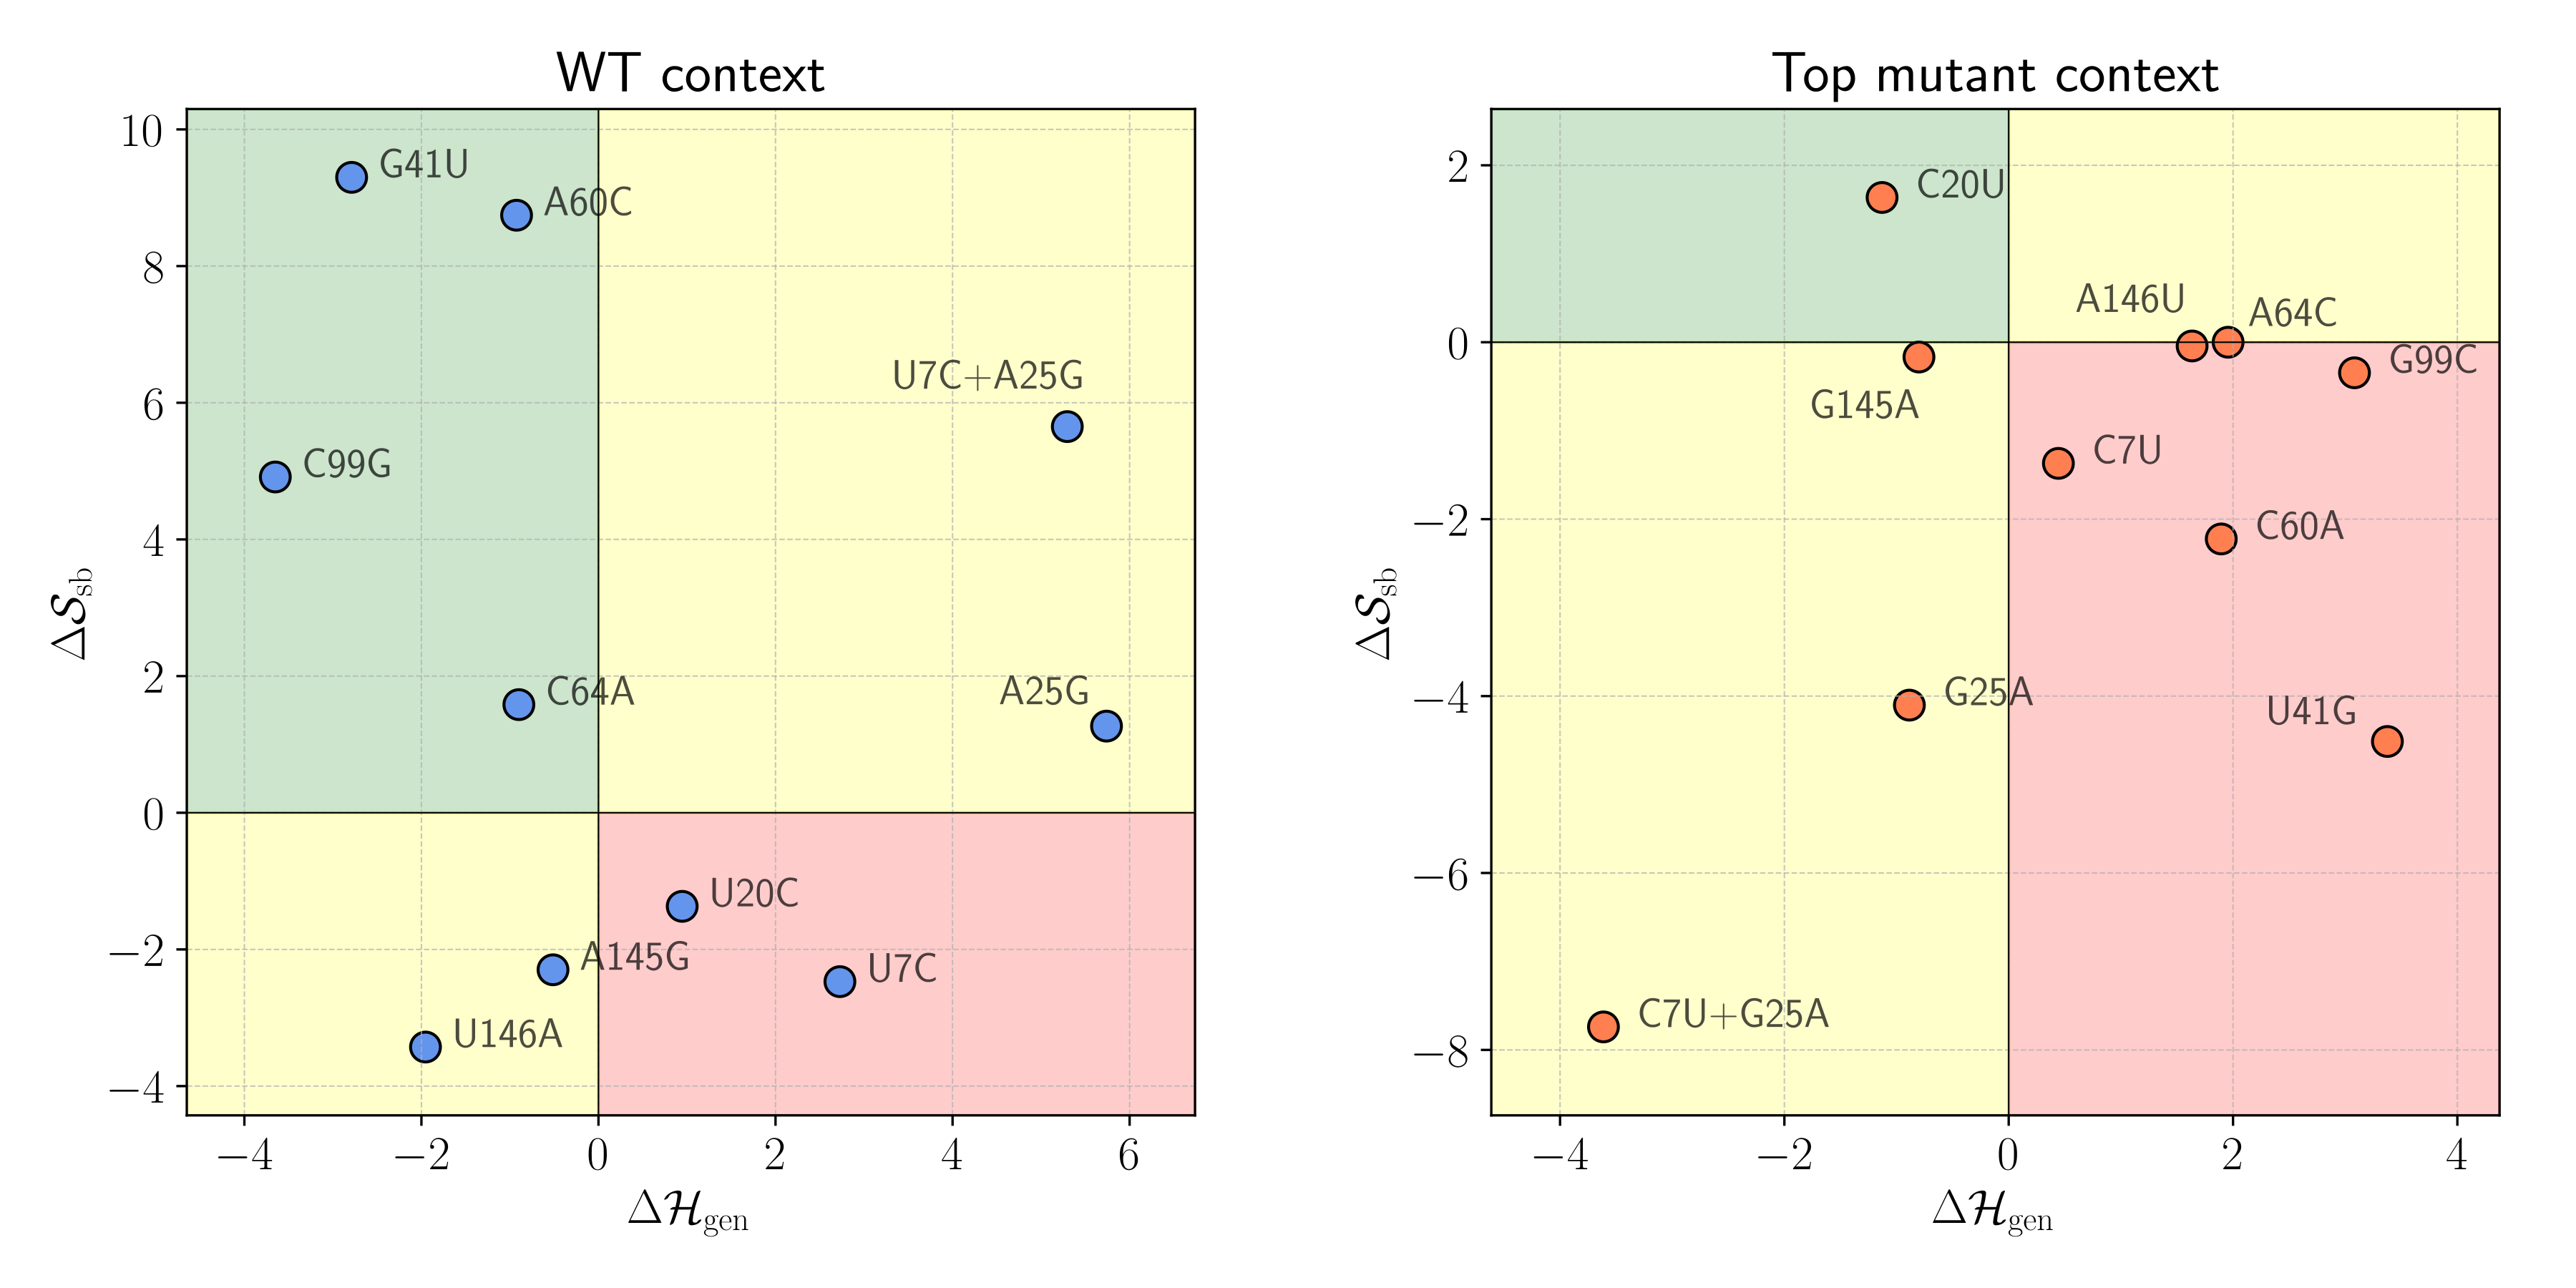
\includegraphics[width=\textwidth]{figures/wt_5_mutations.png}
    \caption{Visualization of the effect of mutations in wild-type 5 in terms of $\Delta \mathcal{S}_{\mathrm{sb}}$ and $\Delta \mathcal{H}_{\mathrm{gen}}$ in the context of the wild-type (left) and the best mutant (right)}
    \label{fig:mutations wt_5}
\end{figure}

\begin{itemize}
    \item \textbf{U7C+A25G}: The wild-type displays the non-canonical pair U-C at positions 8 and 24, which does not allow any hydrogen bound and tends to destabilize the structure.
    In most high-activity mutants, we observe the mutation U8G, which introduces three hydrogen bounds through the G-C pair which is expected to stabilize the structure and increase the thermostability of the ribozyme.
    However, in the best mutant we do not observe this mutation, and the U-C pair is mantained. To compensate for that, the mutant displays the double-mutation U7C+A25G, which changes an A-U WC pair (2 hydrogen bounds) in a G-C pair (3 hydrogen bounds).
    From Fig.~\ref{fig:mutations wt_5} we can see that the mutation U7C alone would sensitively increase the DCA energy and also decrease a bit the SB score.
    The mutation A25G alone is very deleterious in terms of DCA energy, but sensitively improves the BP score.
    When coupling the two mutations, we observe a strong increase of the BP score, although the DCA energy increases. Therefore, this is a BP score induced double mutation.

    \item \textbf{U20C}: This is another rare mutation that is found in the best mutant. It changes the WC pair A-U in a A-C, removing the double hydrogen bound and enlarging the internal loop.
    In the WT context, this mutation is deleterious in terms of DCA energy, but it slightly increases the BP score.
    Instead, in the context of the best mutant, the reversed mutation C20U is beneficial for both scores, suggesting that it is a quite unstable, and probably noise-induced, mutation.

    \item \textbf{G41U}: This is a very important mutation that is observed in almost all high-activity mutants.
    It drastically improves the SB score while also decreasing the DCA energy. Since site 41 is part of a single-stranded region, this mutation can't be explained in terms of WC pairs or deduced from the consensus secondary structure.
    The explanation for this mutation might be found by looking at the tertiary structure. For instance, this site might form a WC pair
    with some residue elsewhere in the structure, or it might be found in a hinge that benefits from additional local flexibility (G is bulky and rigid, U is smaller).
    Fig.~\ref{fig:wt_5 G41X and C99X} (left) shows the frequency of each mutation in the mutants for this site, confirming that the mutation G41U is by far the most common one.

    \item \textbf{A60C}: This mutation stabilizes the structure by replacing the non-canonical pair A-G with a strong G-C WC pair.
    
    \item \textbf{C64A}: This mutation adds an A in the hairpin loop. We observe that this mutant has a lot of A's in the two hairpin loops above, whereas Azoarcus has none.
    
    \item \textbf{C99G}: Very common mutation that most of times changes a C in a G in the hairpin loop, improving both the DCA energy and the SB score. In Fig.~\ref{fig:wt_5 G41X and C99X} (right) we show the frequency
    of each mutation in the mutants.
    

    \item \textbf{U146A}: Quite common mutation that changes a U in an A in the hairpin loop, with the tendency of creating a sequence of A's in the loop.
\end{itemize}

\begin{figure}[h]
    \centering
    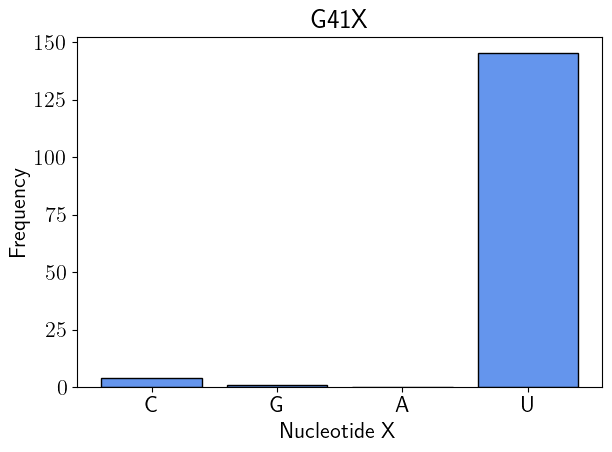
\includegraphics[width=0.45\textwidth]{figures/wt_5-G41X.png}
    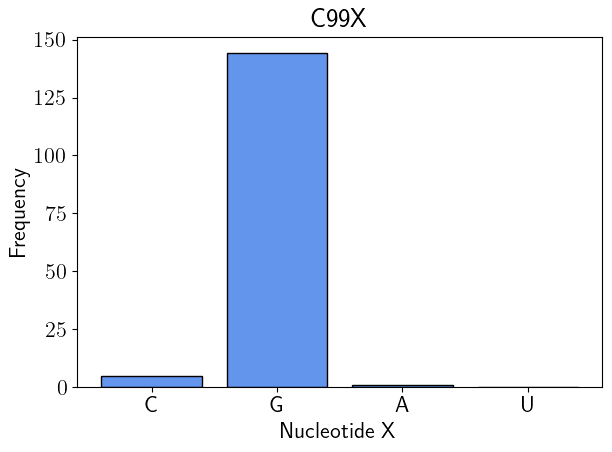
\includegraphics[width=0.45\textwidth]{figures/wt_5-C99X.png}
    \caption{Frequency of each mutation in the mutants for the mutation G41X (left) and C99X (right).}
    \label{fig:wt_5 G41X and C99X}
    \end{figure}

\section{Wild-type 9}
\begin{figure}[h]
    \centering
    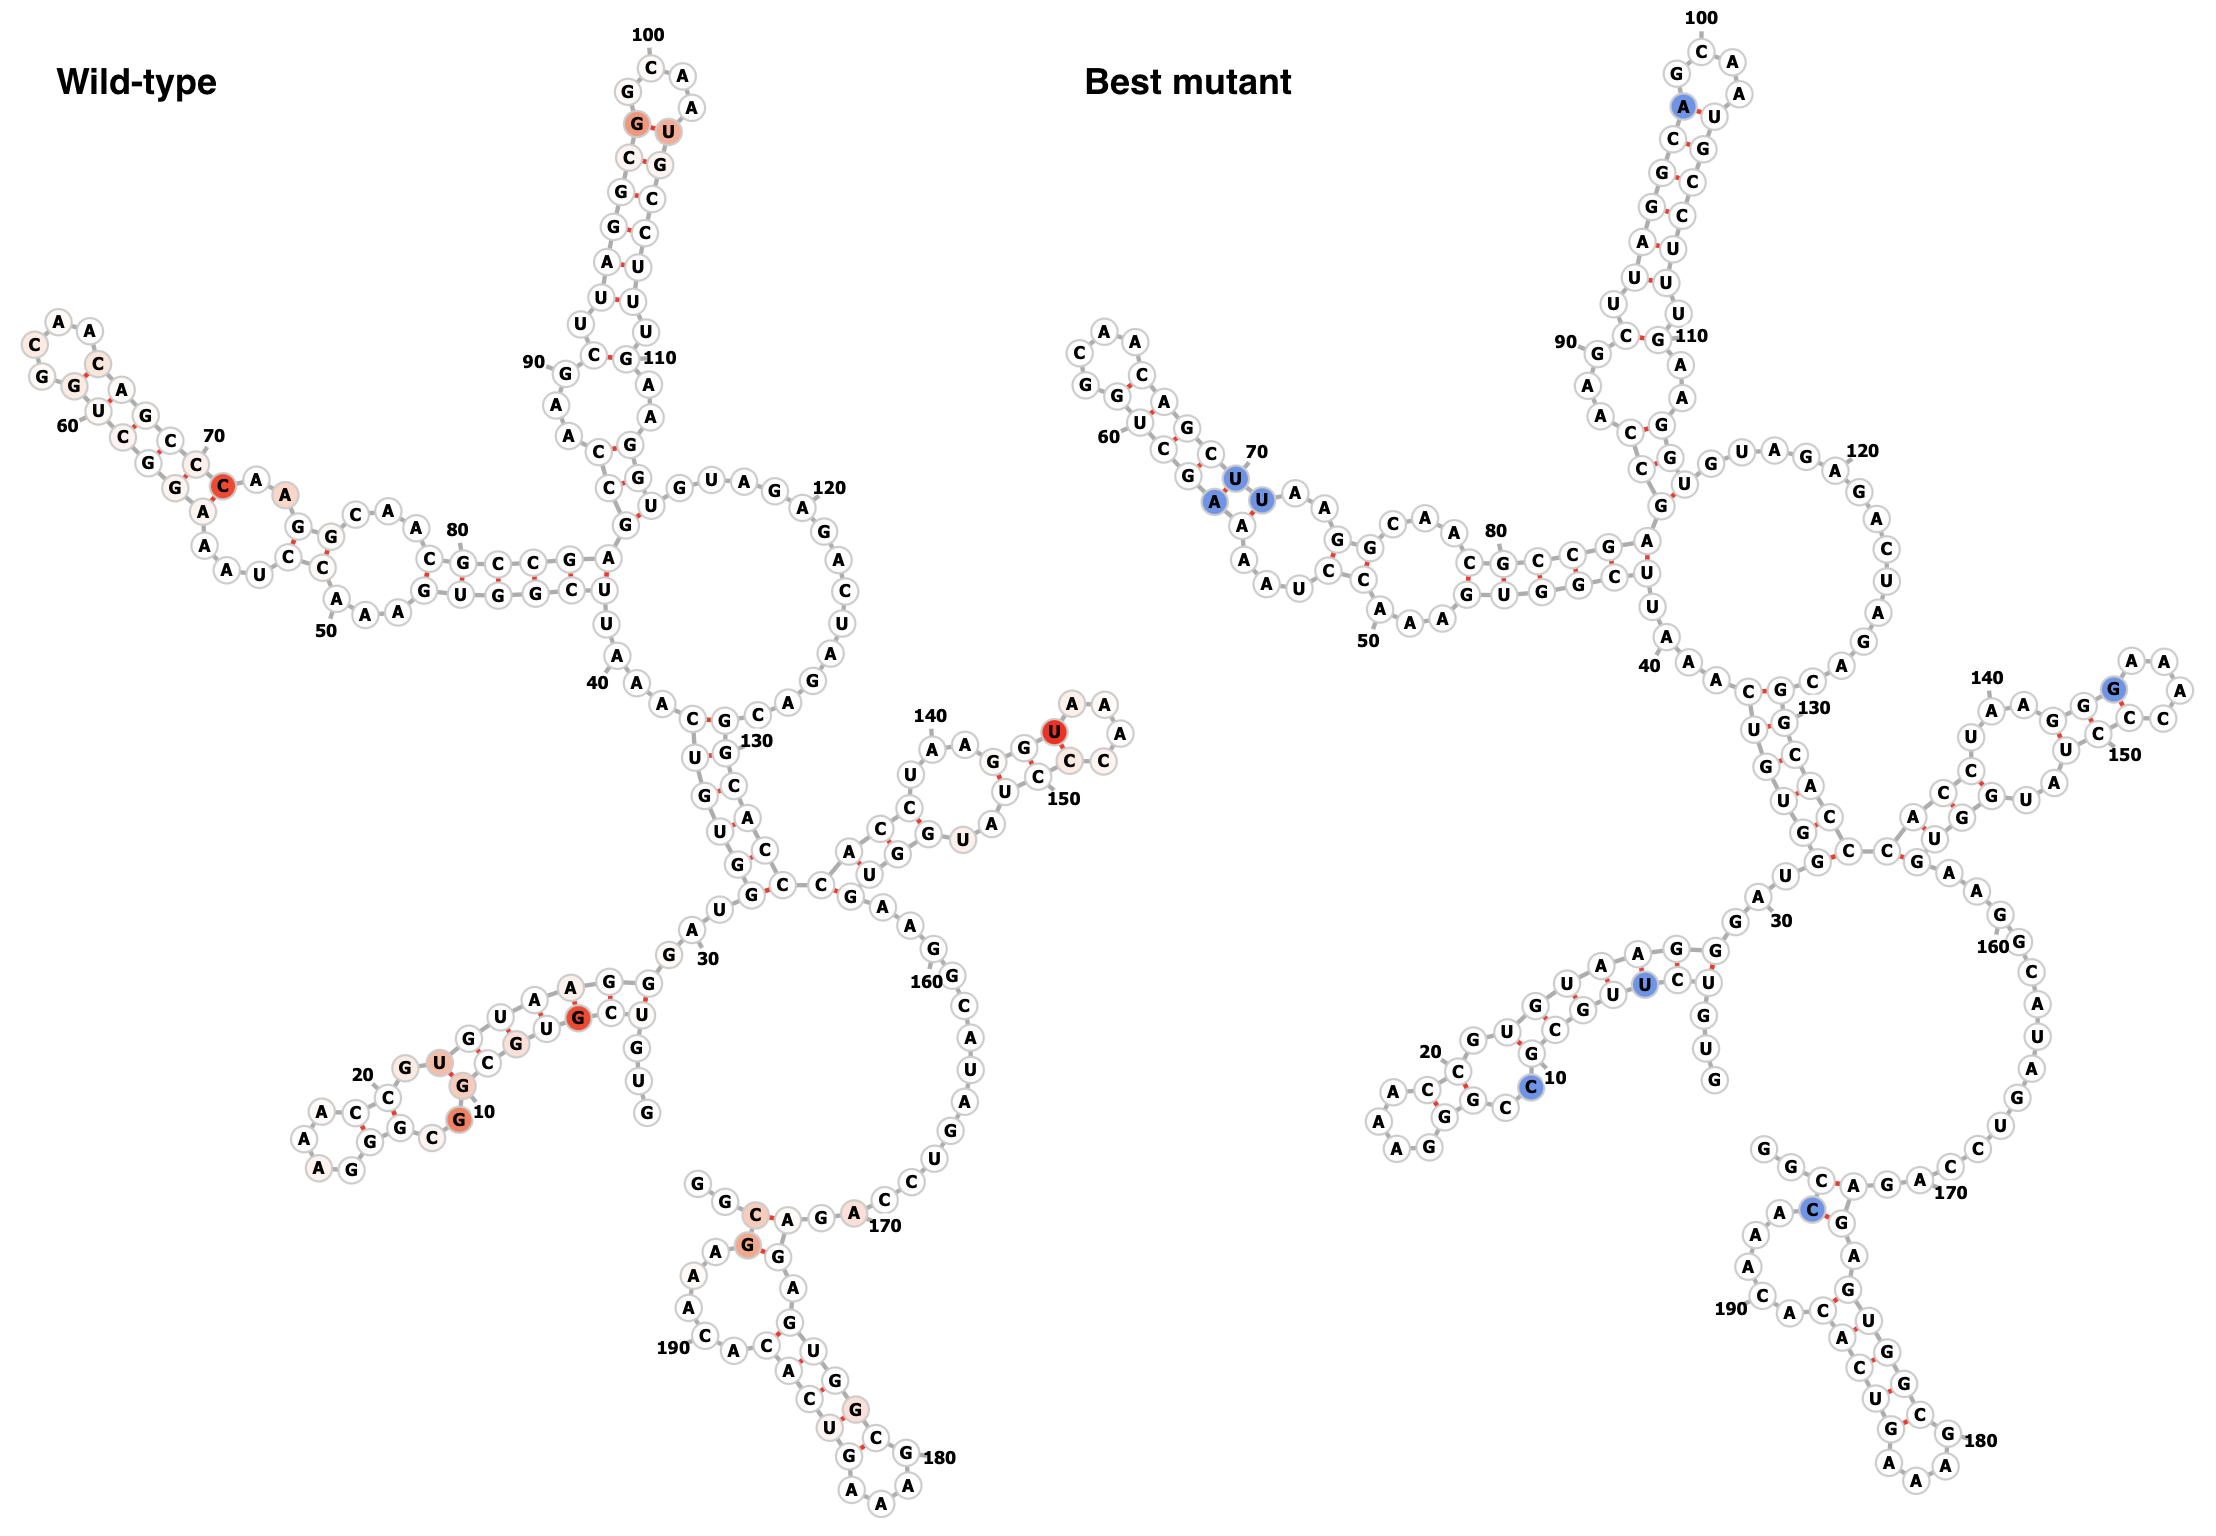
\includegraphics[width=\textwidth]{figures/forna_wt_9.png}
    \caption{Wild-type 9 (left) and the best mutant (right) visualized using the consensus secondary structure.}
    \label{fig:structure wt_9}
\end{figure}

\begin{figure}[h]
    \centering
    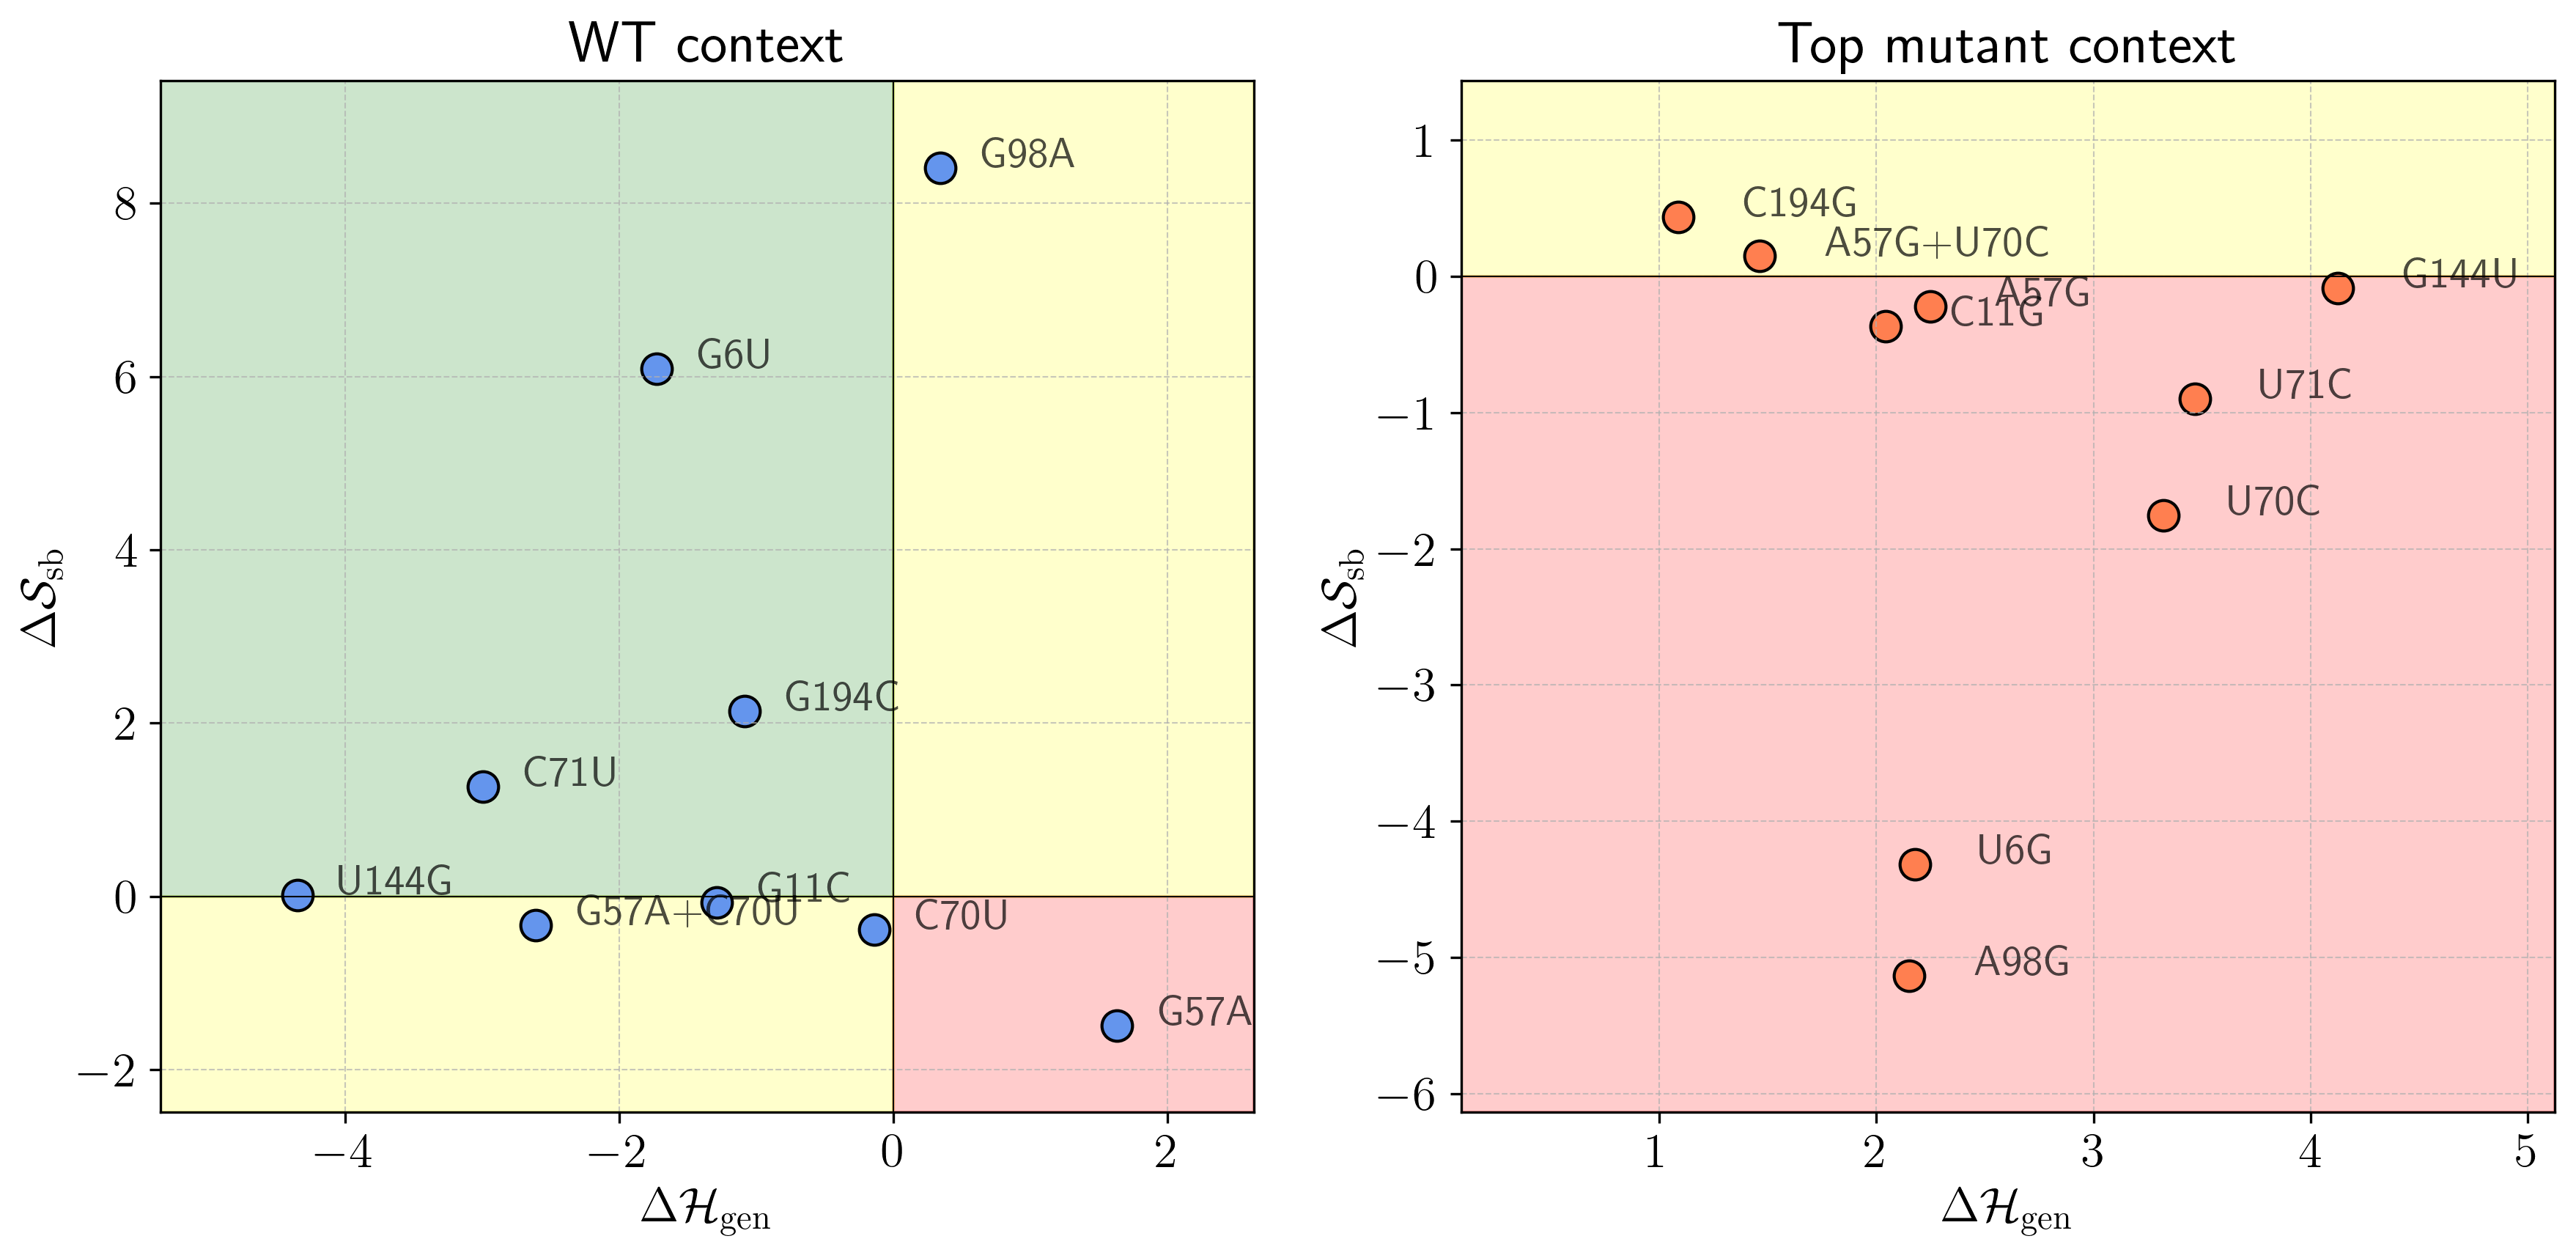
\includegraphics[width=\textwidth]{figures/wt_9_mutations.png}
    \caption{Visualization of the effect of mutations in wild-type 9 in terms of $\Delta \mathcal{S}_{\mathrm{sb}}$ and $\Delta \mathcal{H}_{\mathrm{gen}}$ in the context of the wild-type (left) and the best mutant (right)}
    \label{fig:mutations wt_9}
\end{figure}

Globally, it is interesting to notice (Fig.~\ref{fig:mutations wt_9}, right) that the joint epistatic effect of all the mutations has the effect of fixating each single muatation in the context of the best mutant.
In other words, reverting any single mutation in the best mutant would be deleterious in terms of DCA energy, even for those single mutations (G98A and G57A) that would produce an increasing of the DCA energy if they were introduced in the context of the wild-type.

\begin{itemize}
    \item \textbf{G6U}: Changes a G in a U in the stem, creating an A-U WC pair where before there was an A-G non-canonical pair. This translates in a strong gain in the SB score.
    \item \textbf{G57A + C70U}: This is an interesting double mutation that, unespectedly, sacrifices a strong G-C pair in the stem (G57-C70) to create a weaker A-U pair.
    The mutation G57A alone would be deleterious for both scores, while the mutation C70U alone would be nearly neutral. The co-occurance of the two mutations, insted, is close to neutral in terms of BP score, but very beneficial in terms of DCA energy. Therefore, we observe a strong epistatic effect between these two mutations.
    \item \textbf{C71U}: Changes the A-C pair in between the end of the stem and the beginning of the internal loop in a A-U pair improving both scores, especially the DCA score.
    \item \textbf{G98A}: Creates a A-U pair between the end of the stem and the beginning of the hairpin loop. This mutation is almost neutral in terms of DCA energy, but it is the most beneficial in terms of the SB score.
    \item \textbf{U144G}: This mutation introduces a strong G-C pair right before the hairpin loop. In terms of position it is similar to the mutation G98A, but i is interesting to notice that, while the 
    G98A is very beneficial in terms of SB score, this mutation is neutral for the SB score but the most beneficial in terms of DCA energy.
    \item \textbf{G194C}: Introduces a strong G-C pair for closing the internal loop. It is moderately beneficial for both scores.
\end{itemize}

\end{document}